
\chapter{Error evaluation of interpolation strategies for DCF in local frame\label{chpt:error-evaluation-interpolation-DCF}}

The error introduced by the two interpolation orders for a DCF of
order $n_{\mathrm{max}}=1$ (for which the exact DCF can be computed
directly; see details later) is shown in figure \ref{fig:error}.

\begin{figure}[h]
\centering{}%
\noindent\begin{minipage}[t]{1.1\textwidth}%
\begin{center}
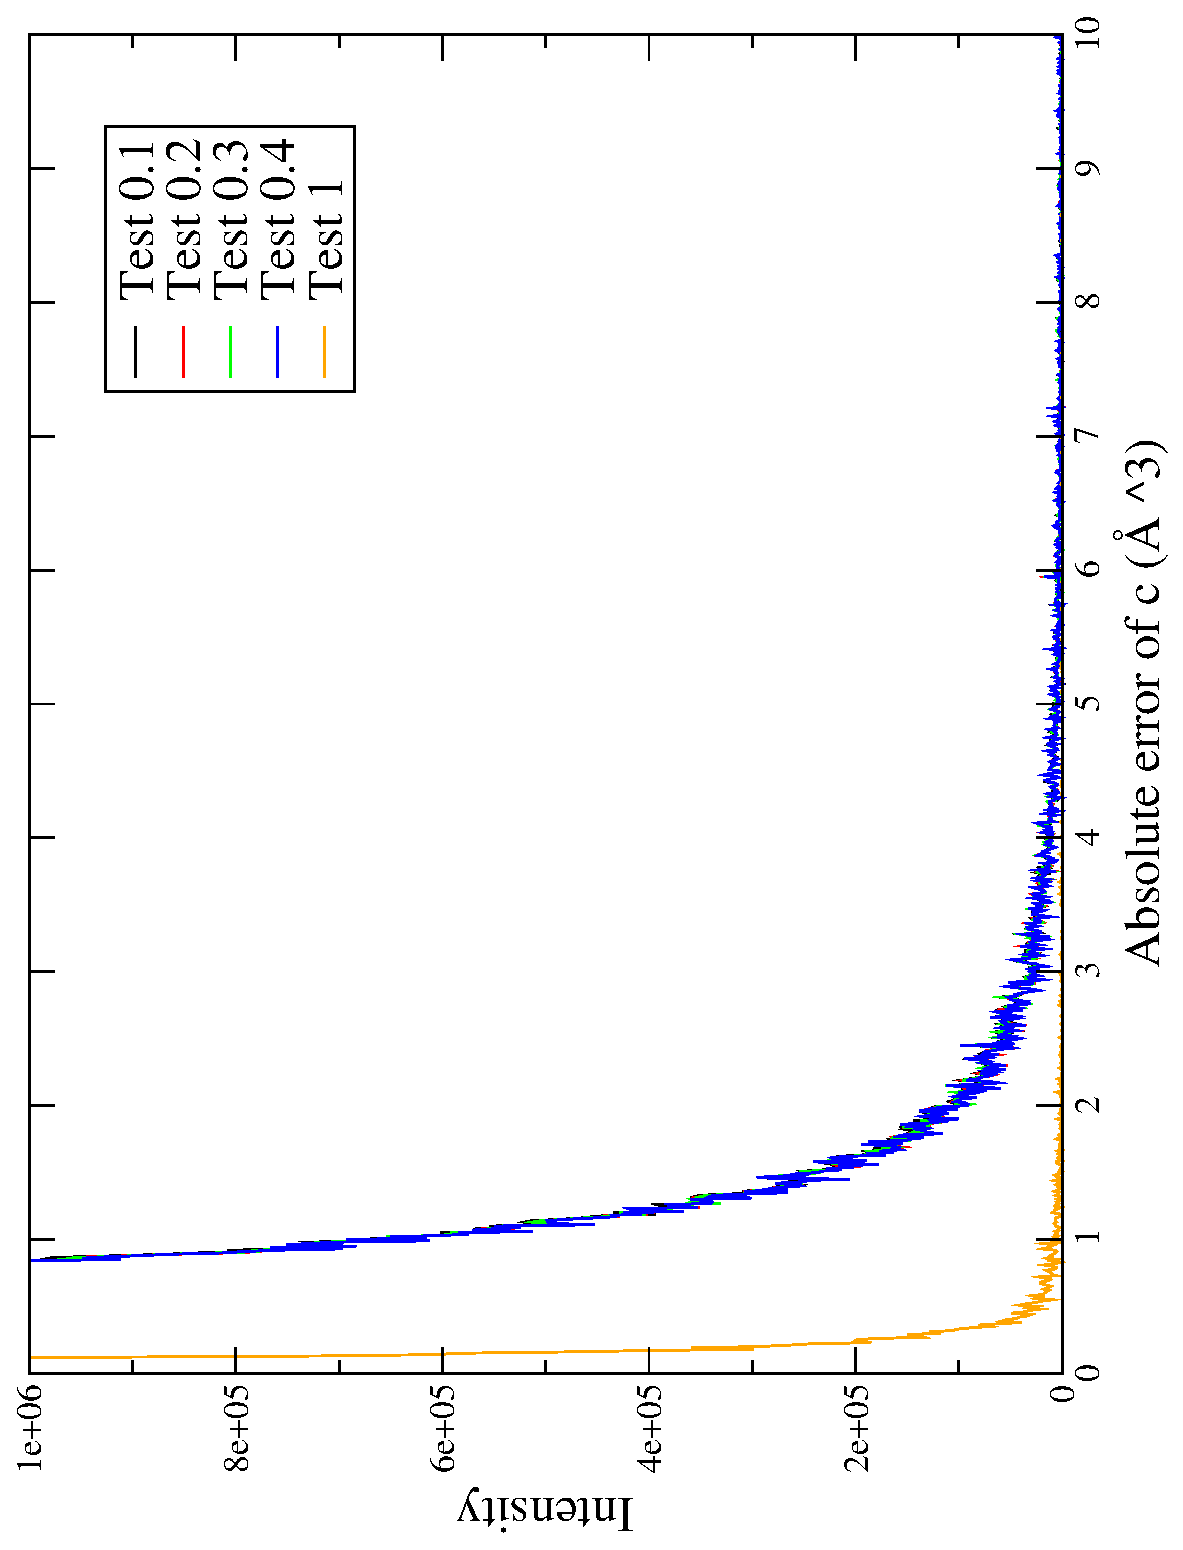
\includegraphics[angle=-90,scale=0.3]{_figure/c_local_to_global_coordinates_32_96/absolute_error}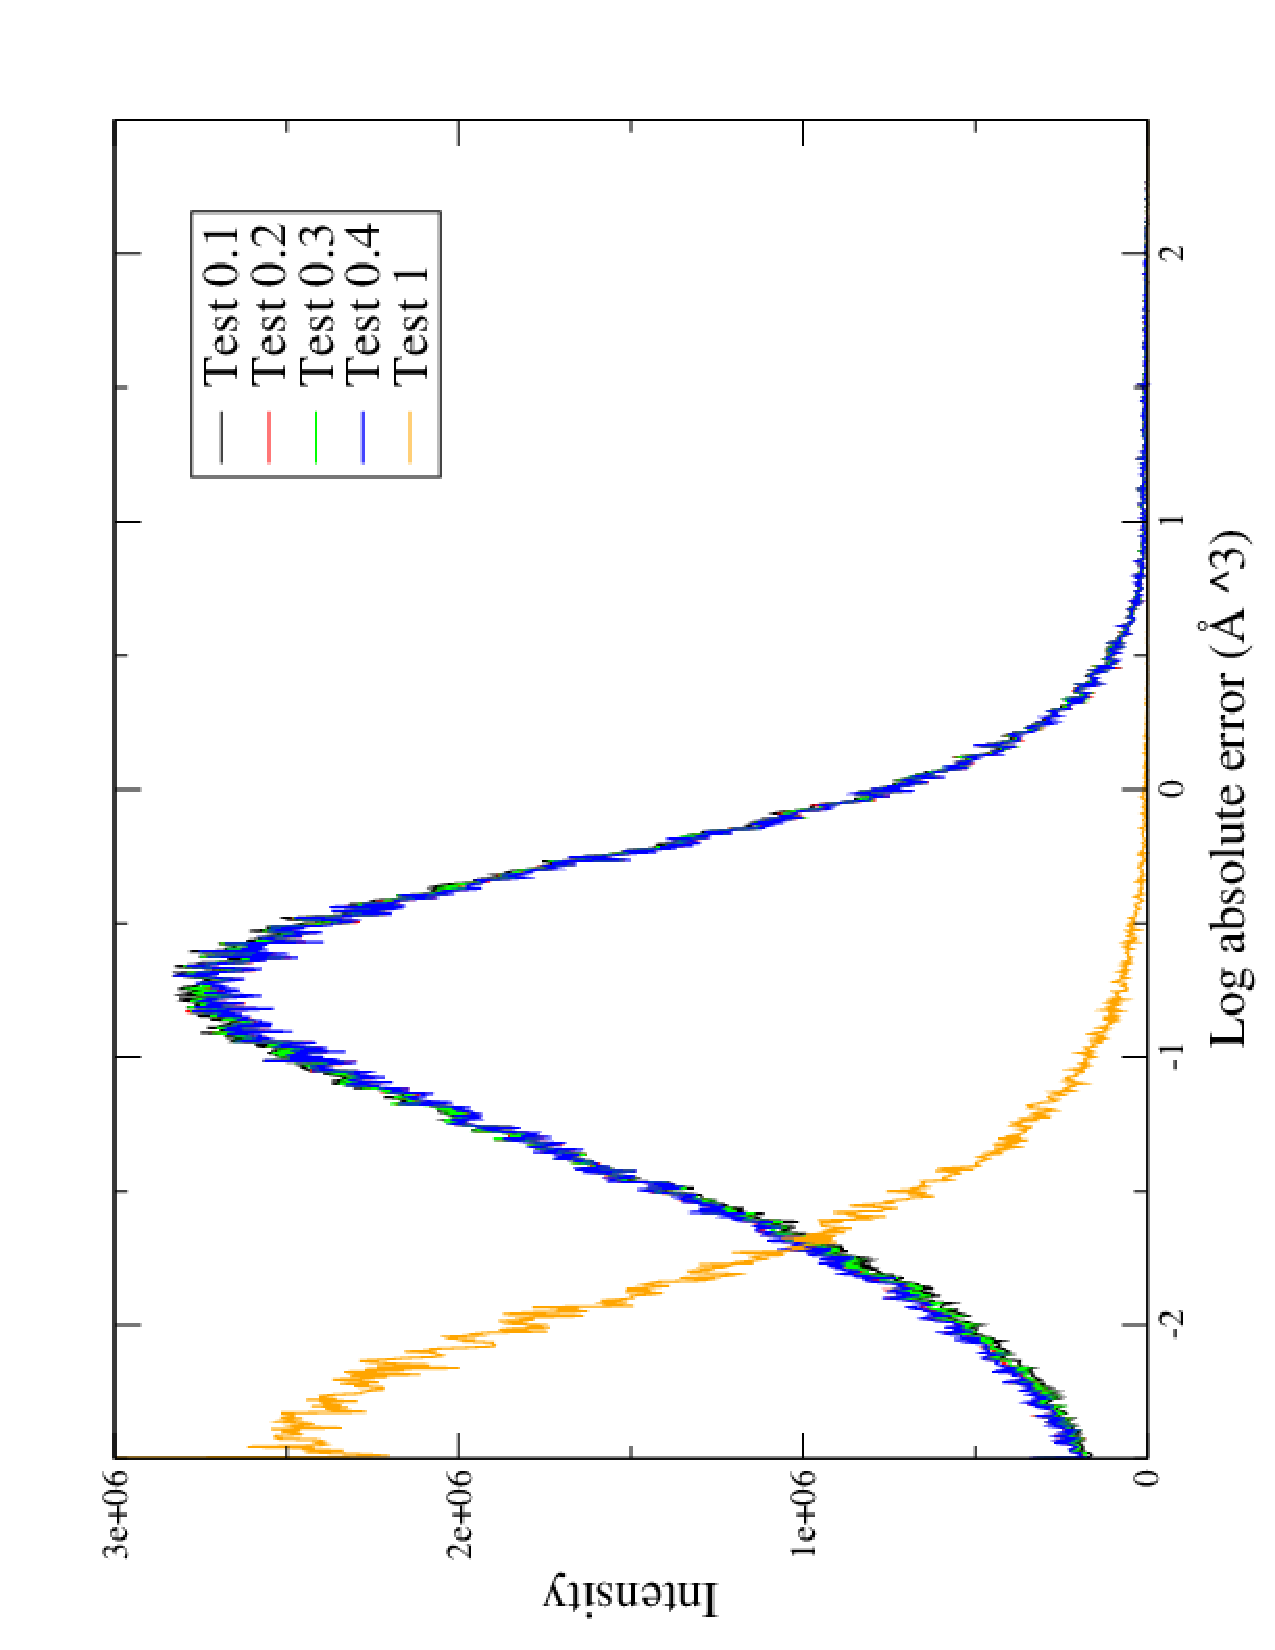
\includegraphics[angle=-90,scale=0.3]{_figure/c_local_to_global_coordinates_32_96/log_absolute_error}
\par\end{center}
\begin{center}
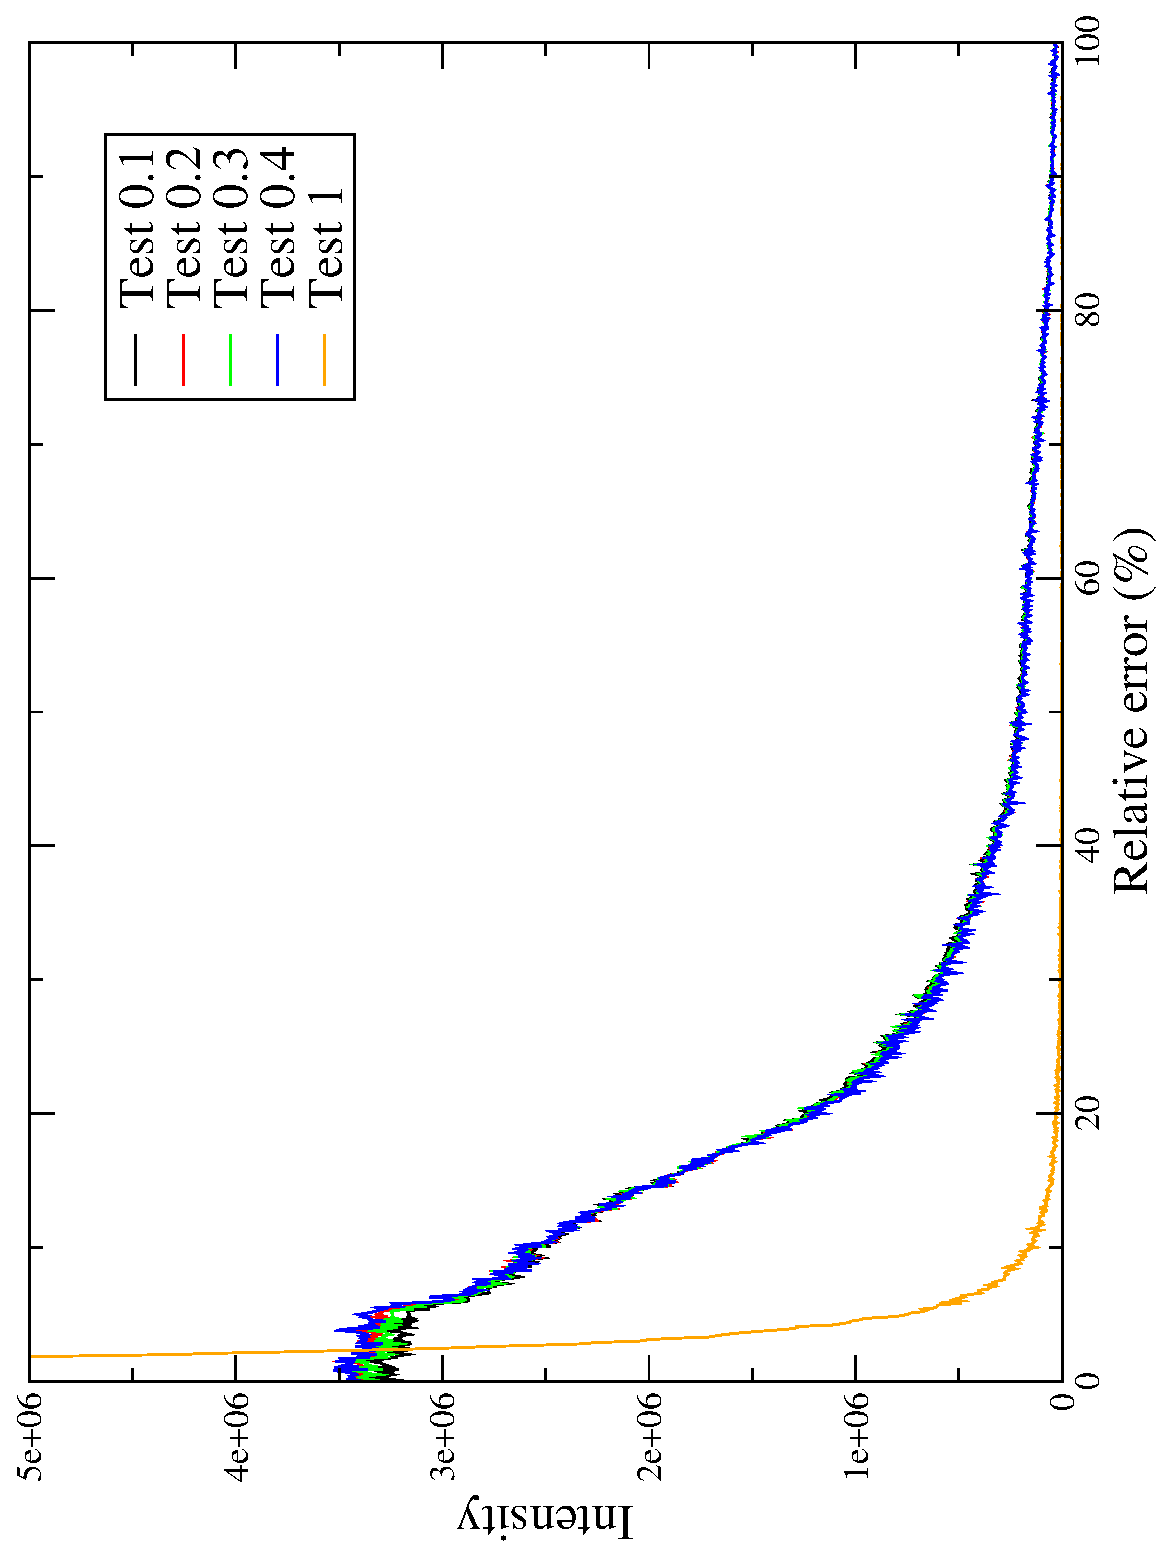
\includegraphics[angle=-90,scale=0.3]{_figure/c_local_to_global_coordinates_32_96/relative_error}
\par\end{center}
\caption[Error of finding $\hat{c}(\mathbf{k},\mathbf{\Omega_{1}},\mathbf{\Omega_{2}})$
by interpolation compared to direct calculation]{Error of finding $\hat{c}(\mathbf{k},\mathbf{\Omega_{1}},\mathbf{\Omega_{2}})$
by interpolation compared to direct calculation: Test 0.1-0.4 is zero
order interpolation with $\phi$ tabulated as in figure \ref{fig:diff_phi}.
Test 1 is linear interpolation.\label{fig:error}}
%
\end{minipage}
\end{figure}

\textbf{Absolute error} is the histogram that counts the number of
times that the calculated DCF gives the corresponding absolute error
$E_{\mathrm{a}}^{i}$ with a resolution of 0.01, in range of $[0,10]$:
\begin{equation}
E_{\mathrm{a}}^{i}=\left|c_{k}^{i}-c_{k}\right|
\end{equation}
where $c_{k}^{i}$ is any element of $\hat{c}(\mathbf{k},\mathbf{\Omega_{1}},\mathbf{\Omega_{2}})$
of unity $\lyxmathsym{\AA}^{3}$ calculated as described and $c_{k}$
is the one calculated directly as the reference.

\textbf{Log absolute error} is treated the same way as $E_{\mathrm{a}}^{i}$,
with $E_{\mathrm{l}}^{i}$ defined as
\begin{equation}
E_{\mathrm{l}}^{i}=\log\left|c_{k}^{i}-c_{k}\right|
\end{equation}

\textbf{Relative error} is defined as
\begin{equation}
E_{r}^{i}=\left|c_{k}^{i}-c_{k}\right|/\left|c_{k}\right|\label{eq:Er}
\end{equation}
with resolution of 0.1\%, in range of {[}0, 1{]}.

In all three figures, the 4 curves given by zero order interpolation
do not diverge a great deal compared with the linear interpolation
one. The result of MDFT also shows that zero order interpolation gives
large energy error with a DCF of $n_{\max}=1$, and has convergency
problems in certain cases. We conclude that the linear interpolation
scheme is absolutely necessary. On the other hand, as seen in eq.
(\ref{eq:interpolation}), it is computationally much more expensive
than the simple histogram scheme, as it requires $2^{5}=32$ times
of operations.
